\documentclass[border=10pt]{standalone}

\usepackage{tikz}
\usepackage{tikzsymbols}
\usetikzlibrary{calc,patterns,shapes.geometric}

\def\centerarc[#1](#2)(#3:#4:#5){\draw[#1] ($(#2)+({#5*cos(#3)},{#5*sin(#3)})$) arc (#3:#4:#5);}

\begin{document}
	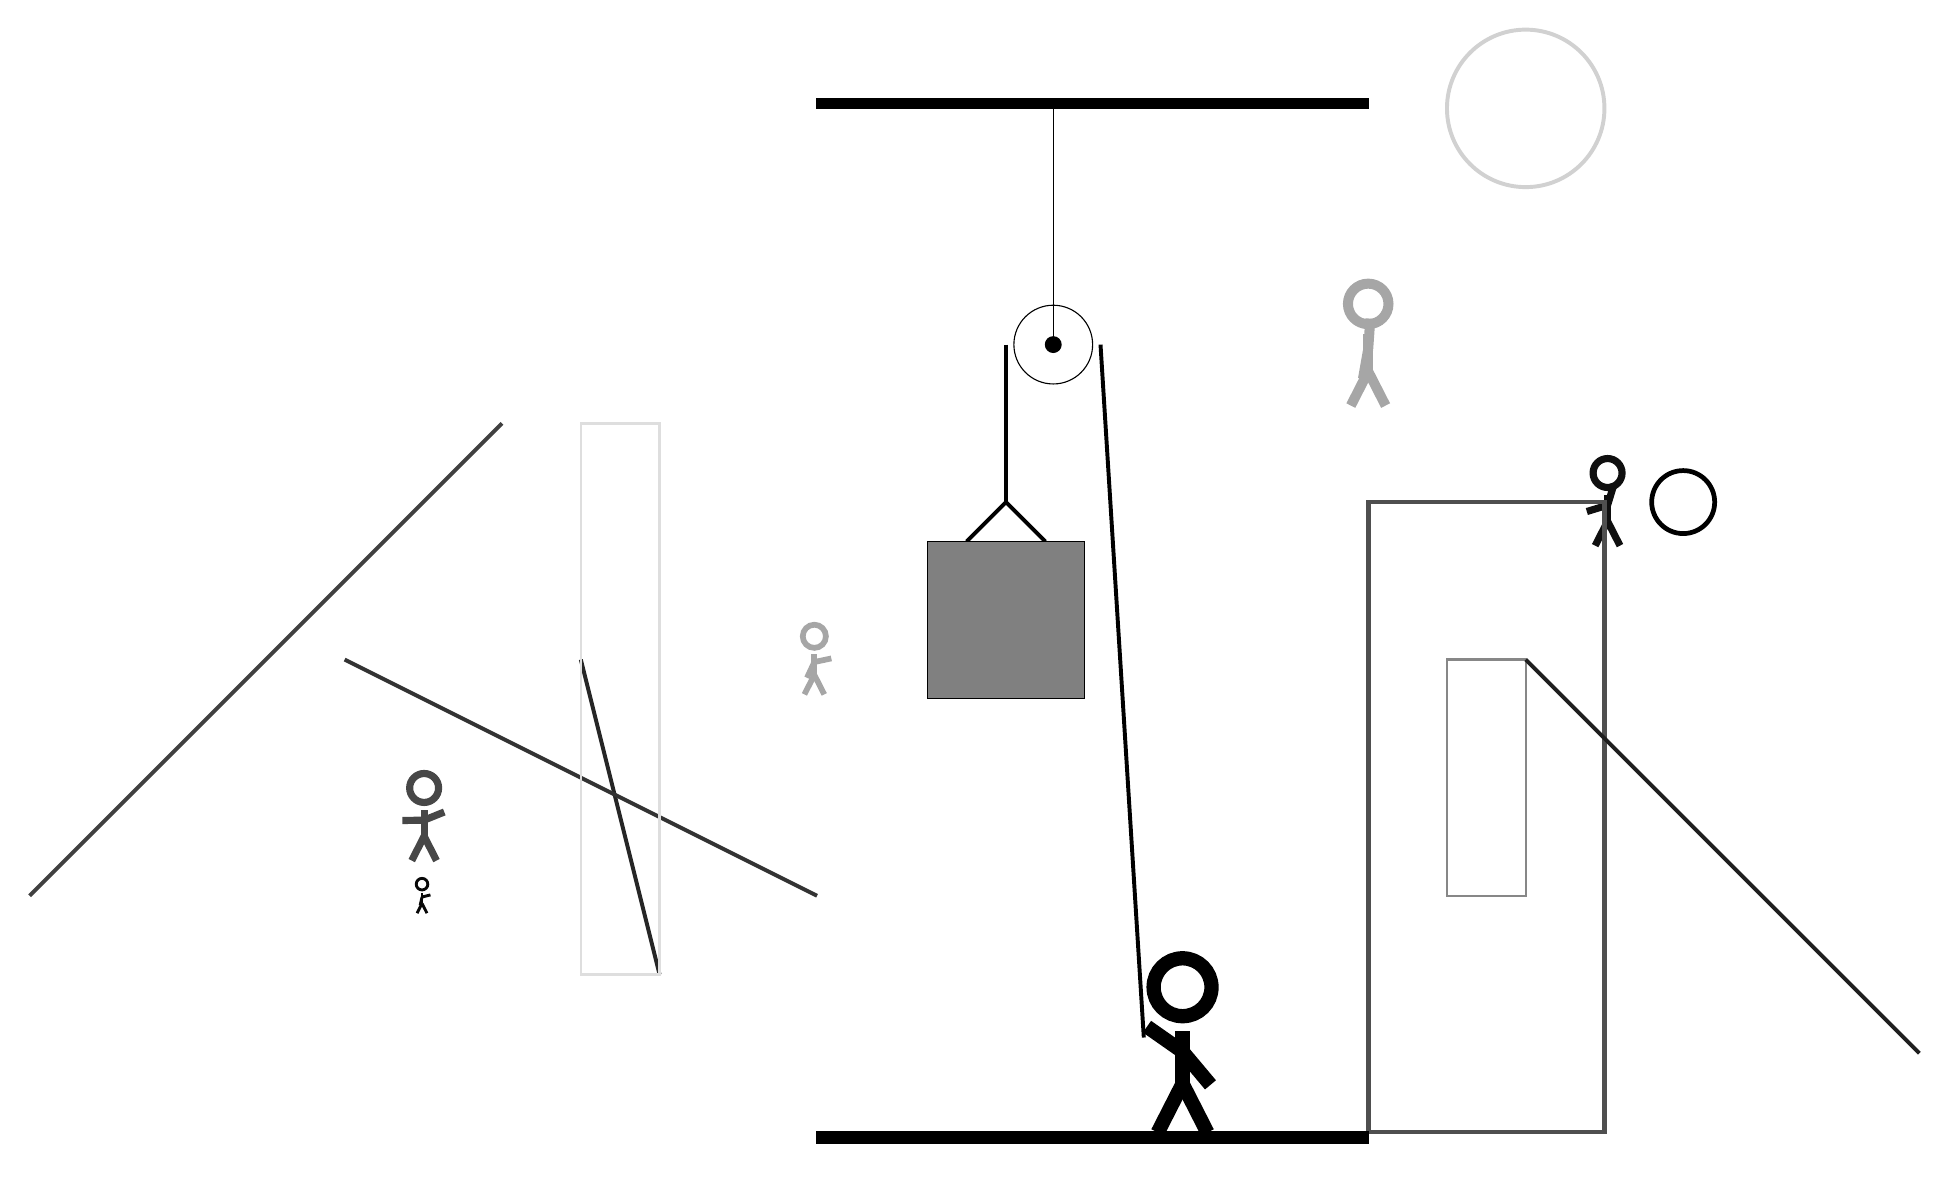
\begin{tikzpicture}
		%%%%% START %%%%%
		
		\draw[fill=black] (-2, 10) rectangle (5, 10.125);
		
		\draw (1, 7) circle (0.5);
		\draw[fill=black] (1, 7) circle (0.1);
		\draw (1, 10) -- (1, 7);
		
		\draw[line width=0.5mm] (-0.1, 4.5) -- (0.4, 5.0) -- (0.9, 4.5);
		\draw[fill=black!50] (-0.6, 4.5) rectangle (1.4, 2.5);
		
		\draw[line width=0.5mm] (0.4, 7) -- (0.4, 5.0);
		\centerarc[line width=0.5mm](1, 7)(0:180:0.6);
		\draw[line width=0.5mm](1.6, 7) -- (2.15, -1.8);
		
		\draw[line width=0.3mm, color=black!47] (7, 3) rectangle (6, 0);
		
		\draw [line width=0.5mm, color=black!18](7, 10) circle (1.0);
		\node[line width=0.7mm, color=black!35] at (-2, 3) {\Strichmaxerl[4][65][12]};
		\node[line width=0.4mm, color=black!94] at (8, 5) {\Strichmaxerl[5][17][73]};
		
		\draw[line width=0.5mm, color=black!75](-6, 6) -- (-12, 0);
		
		\draw[line width=0.6mm, color=black!69] (5, -3) rectangle (8, 5);
		
		\node[line width=0.6mm, color=black!72] at (-7, 1) {\Strichmaxerl[5][1][22]};
		\draw[line width=0.5mm, color=black!85](-4, -1) -- (-5, 3);
		\draw[line width=0.5mm, color=black!88](7, 3) -- (12, -2);
		\draw[line width=0.5mm, color=black!80](-2, 0) -- (-8, 3);
		
		\node[line width=0.5mm, color=black!97] at (-7, 0) {\Strichmaxerl[2][77][14]};
		
		\draw[line width=0.3mm, color=black!13] (-4, -1) rectangle (-5, 6);
		\draw [line width=0.6mm, color=black!100](9, 5) circle (0.4);
		\node[line width=0.5mm, color=black!35] at (5, 7) {\Strichmaxerl[7][80][86]};
		
		\node at (2.6, -1.9) {\Strichmaxerl[10][-35][-50]};
		
		\draw[fill=black] (-2, -3) rectangle (5, -3.15);
		
		%%%%% END %%%%%
	\end{tikzpicture}
\end{document}